% Results of E1, E3 and E4. Every number in this file comes from
%   results/e1_variants.json   (python experiments/e1_variants.py run)
%   results/e1_gold_stats.json (python experiments/e1_variants.py gold-stats)
%   results/e3_retrieval.json  (python experiments/e3_retrieval.py)
%   results/e3_bootstrap.json  (python experiments/e3_retrieval.py bootstrap)
%   results/e4_efficiency.json (python experiments/e4_efficiency.py)

\subsection{E1: Grouping spelling variants}
\label{sec:e1}

\paragraph{Setup.} The 600 gold groups (Section~\ref{sec:gold}) are split into 300 development and
300 test groups (seed 42). The development groups contain 755 strict and 1{,}270 lenient gold pairs,
the test groups 711 and 1{,}267. Each system groups the gold words, and pairwise $P$, $R$ and $F_1$
(Section~\ref{sec:measures}) compare its groups with the gold groups. The systems are exact string
match, lecture Soundex, H-Key with each vowel policy, H-Key with learned variant classes, and the
$k$-means ablation. On the development groups V-norm beat V-drop for plain H-Key (strict $F_1$
0.373 against 0.218), and the best class setting was a V-drop key with $\theta=0.85$ (0.382).
SoundexHindi \citep{kant2020soundexhindi} was not reproduced.

\begin{table}[t]
\centering
\caption{E1 on the 300 test groups: pairwise precision, recall and $F_1$ of each grouping. Strict:
only \textsc{same} pairs are true variants; lenient: \textsc{same} or \textsc{inflection}. Settings
were chosen on the development groups.}
\label{tab:e1}
\small
\begin{tabular}{@{}lccccccc@{}}
\toprule
 & \multicolumn{3}{c}{Strict} & \multicolumn{3}{c}{Lenient} & \\
\cmidrule(lr){2-4}\cmidrule(lr){5-7}
System & $P$ & $R$ & $F_1$ & $P$ & $R$ & $F_1$ & Pairs \\
\midrule
Exact match & 0.000 & 0.000 & 0.000 & 0.000 & 0.000 & 0.000 & 0 \\
Soundex & 0.060 & 0.799 & 0.111 & 0.100 & 0.745 & 0.176 & 9{,}479 \\
H-Key, V-drop & 0.120 & 0.689 & 0.205 & 0.188 & 0.604 & 0.287 & 4{,}073 \\
H-Key, V-norm & 0.452 & 0.301 & \textbf{0.361} & 0.463 & 0.173 & 0.252 & 473 \\
H-Key + classes ($\theta=0.85$) & 0.459 & 0.298 & \textbf{0.361} & 0.470 & 0.171 & 0.251 & 462 \\
H-Key + $k$-means (ablation) & 0.223 & 0.378 & 0.281 & 0.343 & 0.326 & \textbf{0.334} & 1{,}204 \\
\bottomrule
\end{tabular}
\end{table}

\begin{figure}[t]
\centering
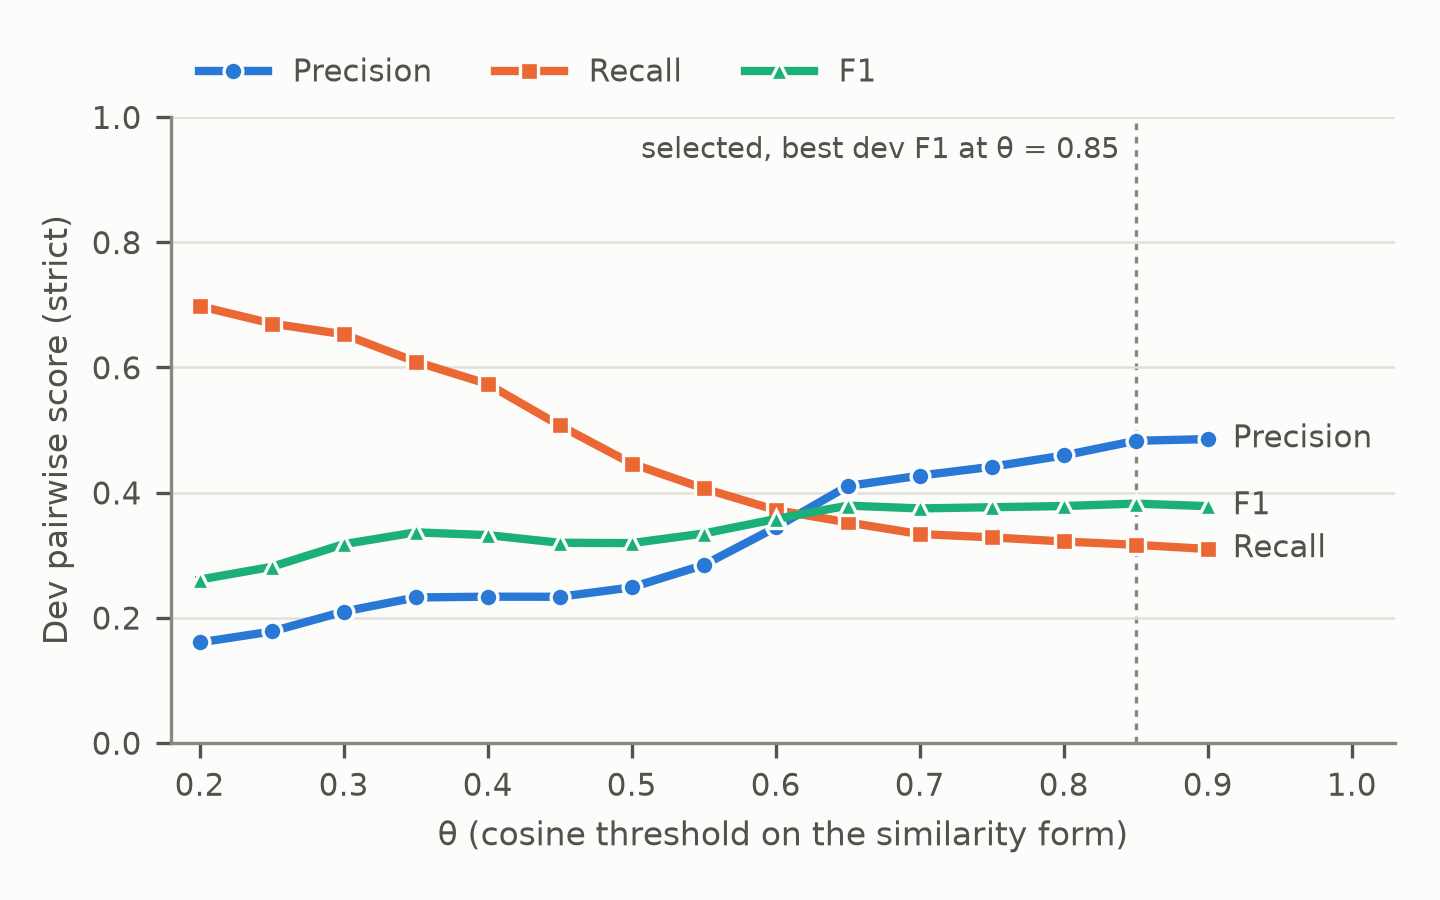
\includegraphics[width=0.75\linewidth]{../figures/e1_theta.png}
\caption{Effect of the merge threshold $\theta$ on the development groups (V-drop key, strict
scores). A low $\theta$ keeps most V-drop merges (high recall, low precision); a high $\theta$ keeps
only words with near-identical similarity forms. With a V-norm key $\theta$ has no effect
(Section~\ref{sec:variants}).}
\label{fig:e1-theta}
\end{figure}

\paragraph{Results.} Table~\ref{tab:e1} gives the test results. Exact match groups nothing, so every
gold pair is a spelling variant that a plain index would miss. Soundex finds most of them (strict
recall 0.799) but puts so many unrelated words together that its precision is 0.060, giving the
lowest $F_1$ of the phonetic systems (0.111). H-Key with V-norm reaches 0.361, more than three times
the $F_1$ of Soundex: it is much more precise (0.452) at the cost of recall (0.301). V-drop sits
between the two, with recall 0.689 and precision 0.120.

The learned classes do not improve on plain V-norm: both reach a strict $F_1$ of 0.361 on test. The
threshold curve (Figure~\ref{fig:e1-theta}) explains why. Starting from V-drop blocks, lowering
$\theta$ trades precision for recall smoothly, and the best development $F_1$ is reached at a high
$\theta$, where only words with nearly identical similarity forms are merged; such classes are
close to V-norm keys. The $k$-means ablation splits large V-drop blocks less strictly: it has the
best lenient $F_1$ (0.334) but a lower strict $F_1$ (0.281), because many of the extra pairs it
forms are inflections rather than spellings of the same form.

\paragraph{Precision is a lower bound.} The scorer treats any two words from different gold groups
as non-variants, although these pairs were never labelled. For H-Key with V-norm on test, 129
false-positive pairs join words from different groups and 130 lie within one group; some of the
former may be true variants, so the true precision of every system is at least the value shown.

\subsection{E3: Retrieval with respelled queries}
\label{sec:e3}

\paragraph{Setup.} Each of the 100 queries (Section~\ref{sec:gold}) respells words of one target
test tweet. Every system indexes all 20{,}000 SentiMix tweets under its mode and ranks them by
lnc.ltc cosine against the query, normalised with the same mode; only the target tweet is relevant.
H-Key with V-drop is included as an ablation, as decided before the first run.

\begin{table}[t]
\centering
\caption{E3: known-item retrieval over 20{,}000 tweets with 100 respelled queries. MAP equals MRR
because each query has one relevant tweet. ``Missed'': queries whose target shares no term with the
query.}
\label{tab:e3}
\small
\begin{tabular}{@{}lcccccc@{}}
\toprule
Index & MRR & P@1 & R@5 & R@10 & MAP & Missed \\
\midrule
Raw & 0.490 & 0.36 & 0.65 & 0.68 & 0.490 & 2 \\
Soundex & 0.762 & 0.66 & 0.89 & 0.95 & 0.762 & 0 \\
H-Key, V-norm (main) & \textbf{0.782} & \textbf{0.69} & \textbf{0.92} & 0.93 & \textbf{0.782} & 1 \\
H-Key + classes & 0.751 & 0.66 & 0.89 & 0.91 & 0.751 & 1 \\
\midrule
H-Key, V-drop (ablation) & 0.810 & 0.71 & 0.93 & 0.98 & 0.810 & 0 \\
\bottomrule
\end{tabular}
\end{table}

\begin{figure}[t]
\centering
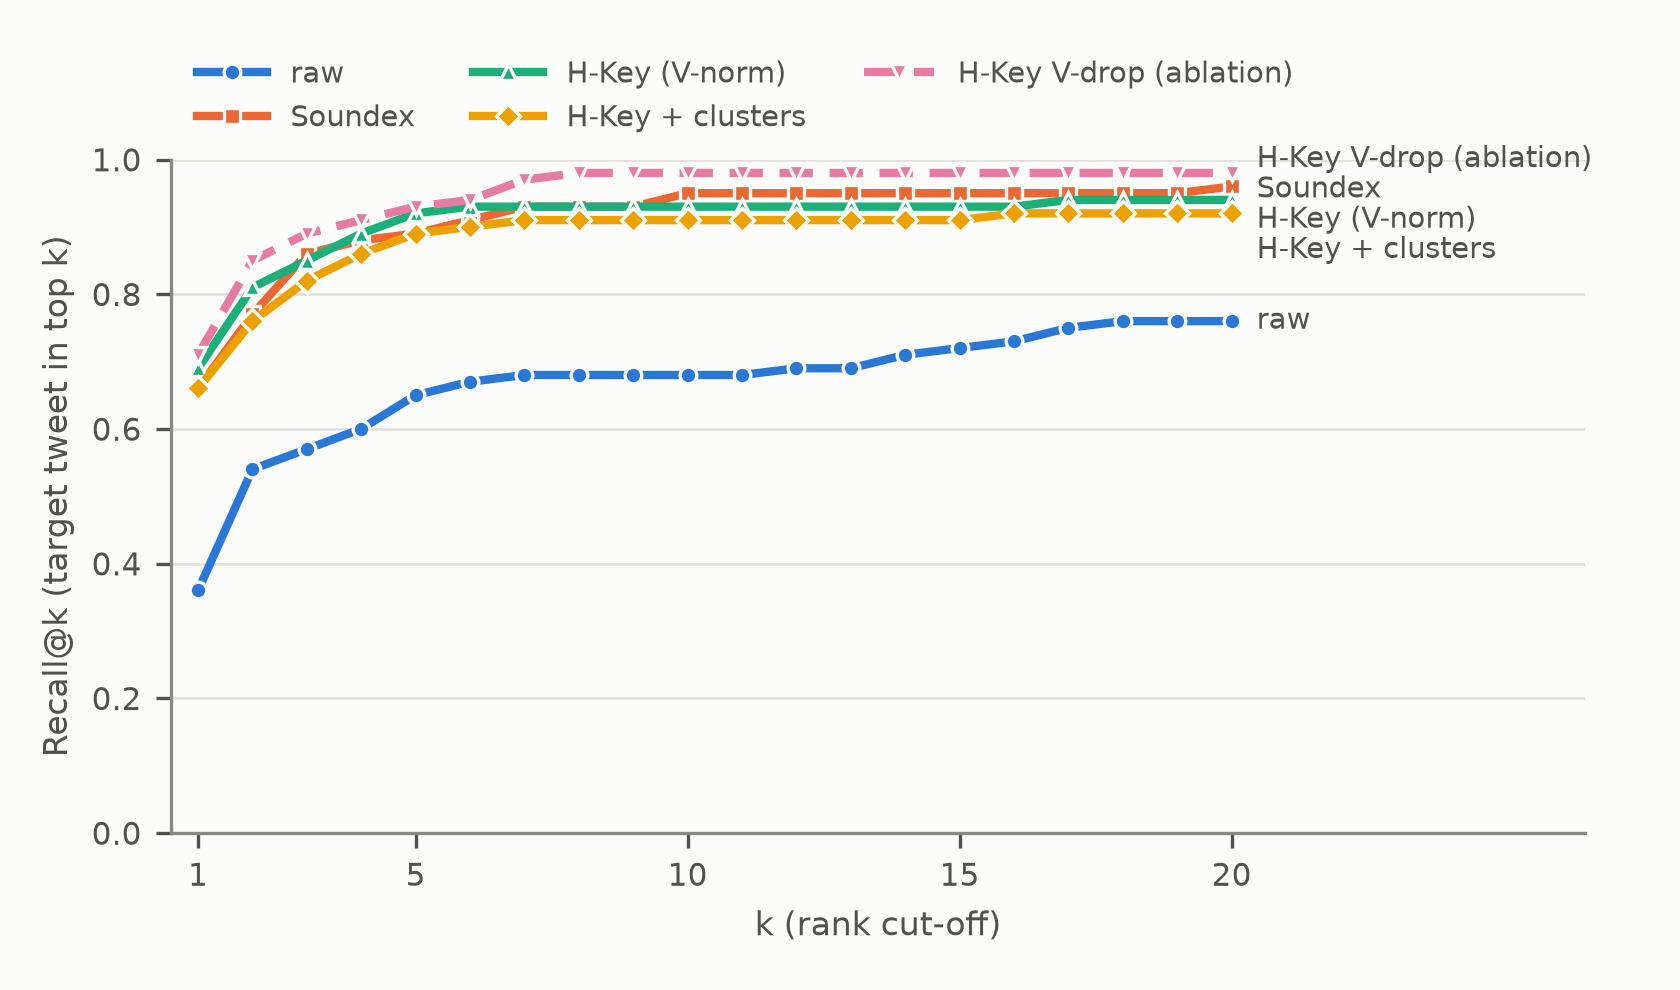
\includegraphics[width=0.8\linewidth]{../figures/e3_recall_at_k.png}
\caption{E3: fraction of queries whose target tweet is in the top $k$, for $k=1,\ldots,20$.}
\label{fig:e3}
\end{figure}

\paragraph{Results.} Normalisation makes a large difference (Table~\ref{tab:e3},
Figure~\ref{fig:e3}). The fraction of queries whose target is ranked first rises from 0.36 with
the raw index to 0.69 with H-Key (V-norm), and the MRR from 0.490 to 0.782. The raw index cannot match a respelled
word at all, so its ranking rests on the words that happen to be spelled the same in query and
tweet. The V-drop ablation is best on every measure (MRR 0.810, R@10 0.98), as its high recall in E1
suggests: query respellings often change vowels (\textit{bahut}$\to$\textit{bohot},
\textit{nahi}$\to$\textit{nhi}), which V-norm keeps apart. Soundex, the worst grouping in E1, is
close behind (MRR 0.762): in known-item search an over-merged term costs little, because the other
query terms still single out the tweet. The learned classes again add nothing over V-norm.

\begin{table}[t]
\centering
\caption{E3 significance: paired bootstrap of the MRR difference over the 100 queries (1{,}000
resamples, seed 42, the same resamples for every row; comparisons fixed before computing).
$p$ is one-sided against \texttt{raw} and two-sided between normalised indexes, uncorrected for
multiple comparisons.}
\label{tab:e3-boot}
\small
\begin{tabular}{@{}lccc@{}}
\toprule
Comparison & $\Delta$MRR & 95\% interval & $p$ \\
\midrule
Soundex $-$ raw & $+0.272$ & $[+0.184,\ +0.367]$ & $<0.001$ \\
H-Key (V-norm) $-$ raw & $+0.292$ & $[+0.216,\ +0.370]$ & $<0.001$ \\
H-Key + classes $-$ raw & $+0.261$ & $[+0.185,\ +0.337]$ & $<0.001$ \\
H-Key V-drop $-$ raw & $+0.320$ & $[+0.240,\ +0.399]$ & $<0.001$ \\
\midrule
H-Key (V-norm) $-$ Soundex & $+0.021$ & $[-0.067,\ +0.093]$ & 0.574 \\
H-Key V-drop $-$ H-Key (V-norm) & $+0.027$ & $[-0.027,\ +0.083]$ & 0.308 \\
H-Key + classes $-$ H-Key (V-norm) & $-0.031$ & $[-0.062,\ -0.007]$ & 0.018 \\
\bottomrule
\end{tabular}
\end{table}

\paragraph{Significance.} Table~\ref{tab:e3-boot} tests these differences with the paired bootstrap
used for E2. Every normalised index beats the raw index: none of the 1{,}000 resamples favours
\texttt{raw}, and every interval lies far above zero, so these gains survive any correction for the
seven tests. Among the normalised indexes, 100 queries cannot separate H-Key from Soundex or the
V-drop ablation from V-norm: both intervals include zero. The learned classes are slightly
\emph{worse} than plain V-norm (interval $[-0.062,-0.007]$), but with $p=0.018$ this does not survive
a Bonferroni correction for the seven tests (threshold $0.05/7\approx0.0071$). The safe conclusion is
that phonetic normalisation of any of these kinds helps retrieval of respelled queries a great deal,
while the choice among them matters little at this sample size.

\subsection{E4: Efficiency}
\label{sec:e4}

\paragraph{Setup.} All five indexes cover the same 20{,}000 tweets (341{,}759 tokens, read in the
order train, dev, test). Query time is measured for the 100 E3 queries (tokenise, normalise, score,
top 10 from the heap), as the median of five runs per query, on one CPU core.

\begin{table}[t]
\centering
\caption{E4: index statistics over 20{,}000 tweets and query time per query (milliseconds).
$b$: exponent of the Heaps' law fit $V=kT^b$.}
\label{tab:e4}
\small
\begin{tabular}{@{}lrrrrrrc@{}}
\toprule
Index & Vocabulary & vs.\ raw & Postings & MB & Median & Max & $b$ \\
\midrule
Raw & 37{,}485 & 1.000 & 317{,}519 & 3.91 & 2.59 & 8.02 & 0.647 \\
Soundex & 4{,}756 & 0.127 & 295{,}313 & 3.33 & 11.94 & 22.50 & 0.367 \\
H-Key, V-norm & 30{,}863 & 0.823 & 316{,}888 & 3.82 & 3.02 & 8.89 & 0.619 \\
H-Key + classes & 30{,}852 & 0.823 & 316{,}881 & 3.83 & 3.00 & 9.00 & 0.618 \\
H-Key, V-drop & 15{,}709 & 0.419 & 302{,}519 & 3.51 & 8.23 & 19.43 & 0.558 \\
\bottomrule
\end{tabular}
\end{table}

\begin{figure}[t]
\centering
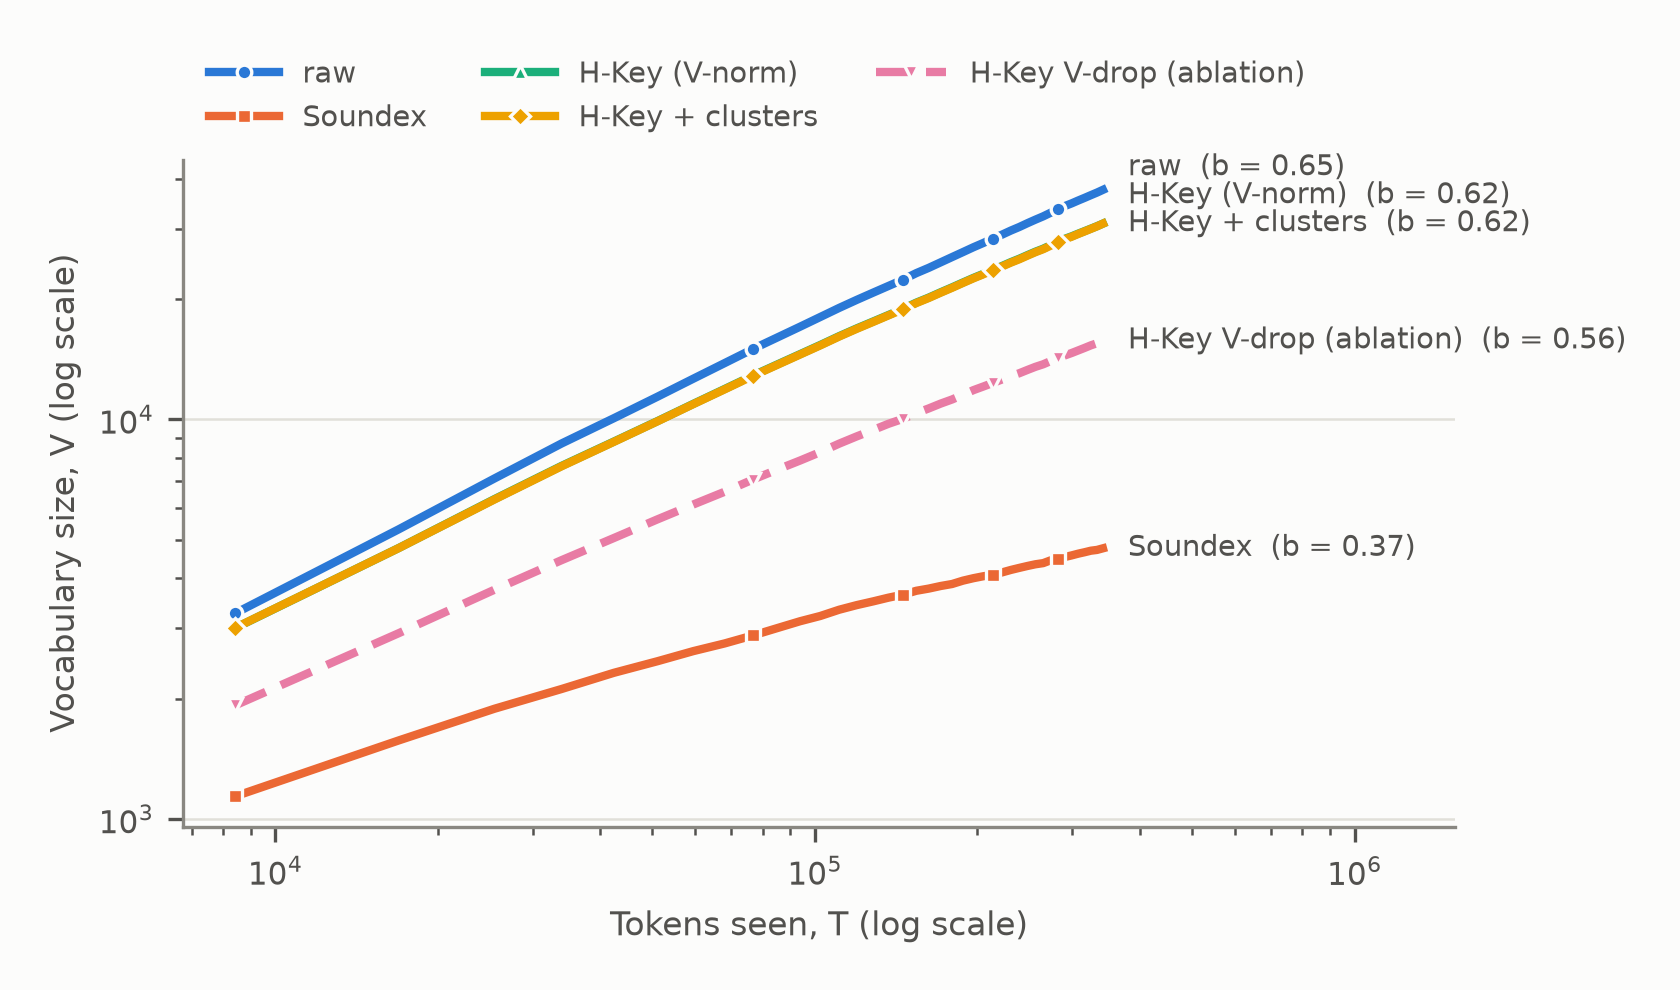
\includegraphics[width=0.8\linewidth]{../figures/e4_vocab_growth.png}
\caption{E4: vocabulary growth as tweets are added (log--log axes) with the fitted Heaps' law
exponent $b$. The H-Key V-norm and class curves coincide.}
\label{fig:e4}
\end{figure}

\paragraph{Results.} H-Key with V-norm shrinks the vocabulary by under a fifth (to 0.823 of raw),
V-drop by more than half (0.419) and Soundex by seven eighths (0.127), see Table~\ref{tab:e4}. The
Heaps' law exponent falls in the same order (raw 0.647, V-norm 0.619, V-drop 0.558, Soundex 0.367;
Figure~\ref{fig:e4}): the coarser the key, the more slowly new terms appear as the collection grows.
The number of postings changes much less than the vocabulary, since merging two terms only merges
their postings within documents that contain both. Fewer terms mean longer postings lists per term,
so coarser keys answer queries more slowly: median 2.59\,ms for raw, 3.02\,ms for V-norm, 8.23\,ms
for V-drop and 11.94\,ms for Soundex. Every index answers every query in at most 22.50\,ms, far
below the 300\,ms interaction budget of the demo, and learning the classes from the training tweets
takes 1.55\,s.
